\subsection{Présentation du système électronique général}
\label{subsec:presentation}

Les systèmes électroniques embarqué à bord des deux étages de la fusée ont été conçus pour être sensiblement similaires, afin de
faciliter le développement, la maintenance et les opérations au sol. Les seuls différences notables entre les deux étages sont
au niveau de la ligne de mise à feu du deuxième étage.

\begin{figure}[h!]
    \centering
    
\includegraphics[width=\textwidth]{figures/elec/Schema_simple.drawio.png}
    \caption{Schéma simplifié du système électronique général de la fusée SP-02}
    \label{fig:schema_electronique_general}
\end{figure}

Le schéma ci-haut (figure \ref{fig:schema_electronique_general}) présente de manière simplifiée les différents éléments du
système électronique général de la fusée SP-02 et leurs interactions.\\

Un schéma amplement plus détaillé est présenté en annexe \ref{subsec:synoptique_fusee}. Ce schéma ne figure pas dans le corps du
rapport pour des raisons de lisibilité, mais est essentiel pour comprendre les différentes interactions entre les éléments du
système électronique et doit être vue comme la synthèse référente principale.

\newpage

\subsubsection{Principaux éléments du système}

On distinguera quatres principaux éléments :
\begin{itemize}
    \item \textbf{\texttt{SEQUENCEUR}} : Responsable de la gestion de tous les événements critiques de la mission et de leur
    synchronisation. C'est lui qui déclenche les différentes étapes de la mission, comme le déploiment des aérofreins, la
    séparation des étages, la commande mise à feu du moteur et le déploiement des parachutes.
    \item \textbf{\texttt{ALLUMAGE}} : Circuit de commande de la ligne de mise à feu du moteur. Son rôle est de fournir la
    puissance nécessaire pour allumer le moteur lorsque le séquenceur l'ordonne et ce en maintenant un niveau de sécurité
    lorsque le moteur n'est pas censé être allumé.
    \item \textbf{\texttt{APEX - APEXeX}} : Comme énoncé plus tôt dans ce document, le projet SP-02 embarquera une carte APEX pour
    réaliser l'ensemble des mesures d'enregistrement et d'envoie par télémesure des données de mission. Elle sera accompagnée
    d'une carte APEXeX\footnote{Parfois également noté ApexEx.}, qui est une extension de la carte APEX, pour permettre
    d'embarquer davantage de capteurs et d'interfaces de communication ainsi que l'ajout d'un module de télémesure supplémentaire.
    Par la suite, dans ce document, nous utiliserons le terme APEX pour faire référence à l'ensemble de la carte APEX et de sa
    carte d'extension APEXeX.
    \item \textbf{\texttt{CAMERA}} : Système de gestion des caméras embarquées, qui comprend la gestion de l'alimentation des
    caméras, leur déclenchement et l'enregistrement de données vidéos.
\end{itemize}

\subsubsection{Interactions entre les éléments du système}

\begin{itemize}
    \item \textbf{\texttt{SEQUENCEUR} $\longrightarrow$ \texttt{SOL}} : Le séquenceur détecte le décollage de la fusée via
    l'arrachange d'un connecteur branché à la rampe de décollage.
    \item \textbf{\texttt{SEQUENCEUR} $\longrightarrow$ \texttt{AEROFREIN}} : Le séquenceur du première étage contrôle le
    servomoteur du système de déploiement des aérofreins.
    \item \textbf{\texttt{SEQUENCEUR} $\longrightarrow$ \texttt{PARACHUTE}} : Chaque séquenceur contrôle le servomoteur du
    système de déploiement du parachutes de l'étage dans lequel il se trouve.
    \item \textbf{\texttt{SEQUENCEUR} $\longrightarrow$ \texttt{SEPARATION}} : Le séquenceur du première étage contrôle le
    servomoteur du système de séparation.
    \item \textbf{\texttt{SEQUENCEUR} $\longrightarrow$ \texttt{ETAGE}} : Chaque séquenceur est branché à un circuit passant par
    l'étage dans lequel il ne se trouve pas. Ainsi, lors de la séparation, ce circuit s'ouvre ce qui permet la détection  de la
    séparation.
    \item \textbf{\texttt{SEQUENCEUR} $\longrightarrow$ \texttt{ALLUMAGE}} : Lorsque le séquenceur du dexuième étage donne l'odre
    de la mise à feu du deuxième moteur, il envoie un signal au circuit d'allumage.
    \item \textbf{\texttt{SEQUENCEUR} $\longleftrightarrow$ \texttt{APEX}} : Le séquenceur de chaque étage est connecté à APEX de
    son étage respectif, lui permettant de lui envoyer des informations sur la temporalité des événements critiques de la
    mission. Cela permet à APEX d'inclure la date de ces événements à sa chaine de données afin de faciliter l'analyse post-vol.
    La chaine de communication entre le séquenceur et APEX est bidirectionnelle par construction (utilisation d'une liaision
    \acrshort{UART}) ce qui rend possible l'envoi de commandes d'APEX vers le séquenceur, voire du sol vers le séquenceur par radio
    via APEX pour par exemple effectuer de la paramétrisation et des tests au sol en séquence de pré-vol. Cela n'a cependant pas
    été considéré comme une fonctionnalité nécessaire à exploiter pour la campagne C'space de 2027.
    \item \textbf{\texttt{SEQUENCEUR} $\longrightarrow$ \texttt{CAMERA}} : Le séquenceur de chaque étage est connecté au
    système de gestion des caméras de son étage respectif, lui permettant de déclencher les caméras embarquées à des moments clés
    de la mission.
    \item \textbf{\texttt{APEX} $\longrightarrow$ \texttt{CAMERA}} : APEX de chaque étage est connecté au système de gestion des
    caméras de son étage respectif, lui permettant de déclencher les caméras embarquées à distance via des commandes envoyées par
    télémesure depuis le sol, ou de manière autonome en fonction de la logique de vol programmée dans APEX.
    \item \textbf{\texttt{APEX} $\longleftrightarrow$ \texttt{STATION SOL}} : APEX de chaque étage est connecté à la station sol
    via deux modules de télémesures, lui permettant d'envoyer des données en temps réel vers le sol et de recevoir des commandes
    depuis le sol.
\end{itemize}

Ces intéractions sont succinctement présentées dans le schéma de la figure \ref{fig:schema_electronique_general} et y sont
détaillées dans le schéma plus complet présenté en annexe \ref{subsec:synoptique_fusee}.

\subsubsection{Présentation des cartes électroniques}

\begin{table}[h!]
    \centering
    \begin{tabular}{|l|p{2cm}|p{6cm}|c|c|c|}
    \hline
    Catégorie & Nom & Description & Etage 1 & Etage 2 & Total \\ \hline
    \multirow{5}{*}{Expérience} & Apex & Carte principal d'acquisition des données de vol et de logique & 1 & 1 & 2 \\ \cline{2-6}
                                & ApexEx & Carte d'extension d'Apex & 1 & 1 & 2 \\ \cline{2-6}
                                & Pitot & Carte support de capteur de pression de la pointe & 0 & 1 & 1 \\ \cline{2-6}
                                & Caméra & Carte de contrôle des caméras & 1 & 1 & 2 \\
    \hline
    \multirow{3}{*}{Séquenceur} & Séquenceur & Carte séquenceur & 1 & 1 & 2 \\ \cline{2-6}
                                & \acrshort{IHF} & Carte Interface Homme Fusée & 1 & 1 & 2 \\ \cline{2-6}
                                & Allumage principale & Carte servant de logique de puissance et d'interface du système d'allumage & 0 & 1 & 1 \\ \cline{2-6}
                                & Condensateur & Banque des condensateurs du système d'allumage & 0 & 1 & 1 \\
    \hline
    \multirow{2}{*}{Divers} & Connecteur séparation & Connecteur d'interface entre les deux étages & 2 & 0 & 2 \\ \cline{2-6}
                            & Routeur & Carte servant d'interface entre le séquenceur de l'étage, le jack et les connecteurs de la séparation & 1 & 1 & 2 \\
    \hline
    \multicolumn{3}{c|}{} & 8 & 9 & 17 \\
    \cline{4-6}
    \end{tabular}
    \caption{Présentation de l'ensemble des cartes électroniques}
\end{table}

Les cartes électroniques embarquées à bord de la fusée SP-02 sont présentées dans le tableau ci-dessus. L'intégralité des schémas
électriques de ces cartes sont présentés en annexe \ref{subsec:schema_elecs}.

\vfill

\begin{figure}[H]
    \centering
    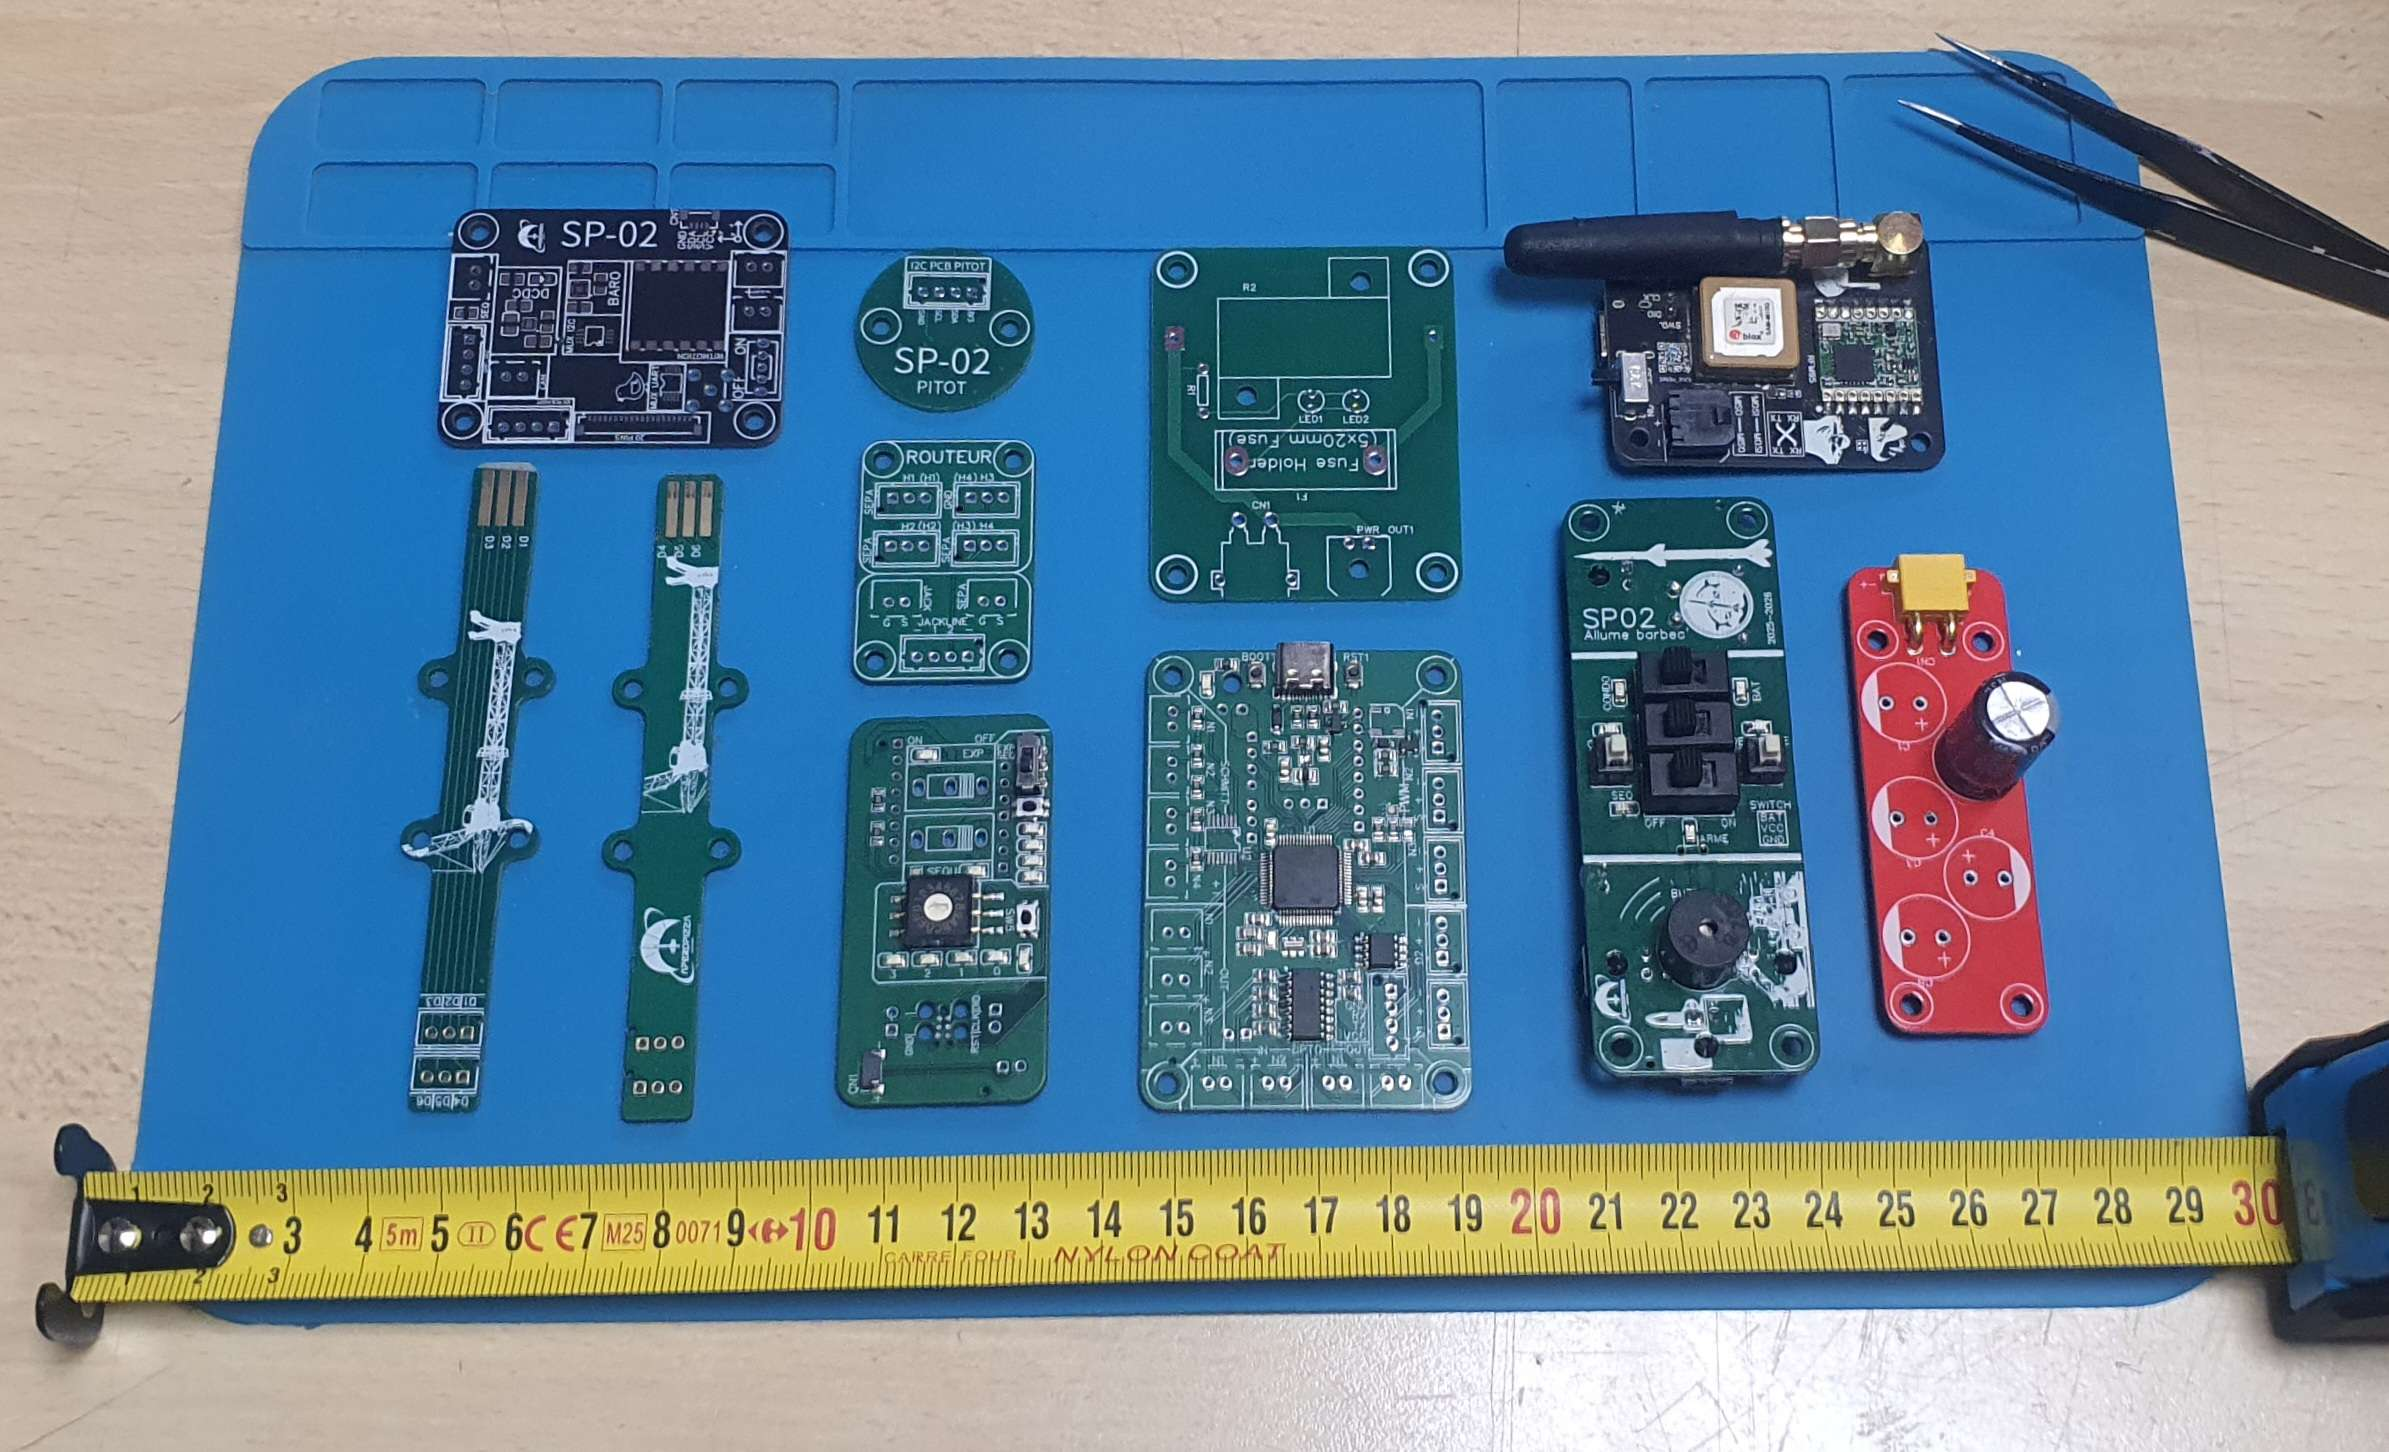
\includegraphics[width=0.9\textwidth]{figures/elec/ensemble_pcbs.jpg}
    \caption{Vue d'ensemble des types de cartes électroniques embarquées à bord de la fusée SP-02}
    \label{fig:ensemble_pcbs}
\end{figure}

La figure \ref{fig:ensemble_pcbs} présente une vue d'ensemble des différents types de cartes électroniques qui ont été
développées. A noter qu'à cette ensemble, il manque la carte caméra, que la carte se situant au dessus du séquenceur n'est pas
cité dans le tableau précédent puisque c'est une carte de test et que la carte condensateur (en rouge) est une ancienne version.

\newpage
